% Number 1
% BFPM Tension FBD Vectors
% Hanging box, rope around 2 pulleys, theta = phi

% Watermark
\AddToShipoutPicture*{\BackgroundPic}

\addtocounter {ProbNum} {1}

\begin{floatingfigure}[r]{.2\textwidth}
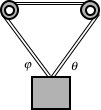
\includegraphics[scale=1]{/Users/jgates/desktop/latex/pics/hangingbox1.png}
\end{floatingfigure}
 
{\bf \Large{\arabic{ProbNum}}} The box of mass ${6~kg}$ hangs at rest. 

\bigskip

\indent  a. Prove that ${\theta = \varphi}$.

\vfill

b. Determine the tension in the rope, if ${\theta = 50^\circ}$.

\vfill

\newpage
